\documentclass{../lab}

\labacronym{MUO}
\labtitle{Muon Lifetime}

%\newcommand{\[1]}{http://experimentationlab.berkeley.edu/node/88}
%\newcommand{\SRSDG645Manual}{http://www.thinksrs.com/downloads/PDFs/Manuals/DG645m.pdf}
%\newcommand{\Physics111LibrarySite}{http://physics111.lib.berkeley.edu/Physics111/Reprints/MUO/MUO_index.html}
%\newcommand{\CosmicRays}{http://physics111.lib.berkeley.edu/Physics111/Reprints/MUO/02-Cosmic-Ray_Phenomena.pdf}
%\newcommand{\RCAPhotoMultiplierTubeManual}{http://physics111.lib.berkeley.edu/Physics111/Equipment_Manuals/RCA_PMT.pdf}
%\newcommand{\Root'smainsite}{http://root.cern.ch}

\begin{document}

\maketitle

\tableofcontents

\section{Description of the Muon Lifetime Experiment (MUO)}

Revised 2017

\begin{enumerate}
    \item \textbf{Note that there is NO eating or drinking in the 111-Lab anywhere, except in rooms 282 \& 286 LeConte on the bench with the BLUE stripe around it.} Thank You the Staff.

\end{enumerate}

The muon is an unstable particle, with a lifetime on the order of microseconds, which decays by means of the weak interaction into an electron and two neutrinos. If we start out with $N_o$ muons, then the number of muons present at a time $t$ later is $N(t) = N_0 e^{-\frac{t}{T}}$ where $T$ is the mean life.

In this experiment, cosmic-ray muons that enter a large tank of liquid scintillator trigger the emission of a pulse of photons. These photons are detected by a photomultiplier tube. If the muon stops inside the tank, another pulse of light is produced when the muon decays. The time difference between the pulses is a mean for measuring the lifetime. An histogram of these time differences for many decaying muons resembles an exponential distribution from which the mean lifetime can be determined.

You will get acquainted with a number of electronic devices that are quite common in laboratories. Data analysis using a computer and program writing are required. You will spend time in setting up the equipment. Once that's done and data-taking is started, you don't need to be in the lab, except for checking out how everything is working.

\begin{enumerate}
    \item Pre-requisites: None

    \item Days Allotted for the Experiment: 6
\end{enumerate}

\noindent\textbf{All pages in this lab. Note To print Full Lab Write-up click on each link below and print separately }

\begin{enumerate}
    \item \textbf{Muon Lifetime}
    
    \item \href{http://experimentationlab.berkeley.edu/node/86}{\textbf{Exponential Probability Distributions}}
    
    \item \href{http://experimentationlab.berkeley.edu/EAX}{\textbf{Error Analysis Notes}}
    
    \item \href{http://experimentationlab.berkeley.edu/node/88}{\textbf{National Instruments Digitizer VI}}
    
    \item \href{http://experimentationlab.berkeley.edu/sites/default/files/DG645manual.pdf}{\textbf{Stanford Research Systems DG645}}
\end{enumerate}

Reprints and other information can be found on the \href{http://physics111.lib.berkeley.edu/Physics111/Reprints/MUO/MUO\_index.html}{\textbf{Physics 111 Library Site}}

This lab will be graded 20\% on theory, 20\% on technique, and 60\% on analysis. For more information, see the \href{\AdvancedLabSyllabus}{\textbf{Advanced Lab Syllabus}}.

Comments: E-mail \href{\MailDonOrlando}{\textbf{Don Orlando}}

\section{Muon Lifetime Experiment Photos}

\begin{figure}[h]
\begin{minipage}{0.24\textwidth}
    \href{http://experimentationlab.berkeley.edu/sites/default/files/images/MUO_3517.jpg}{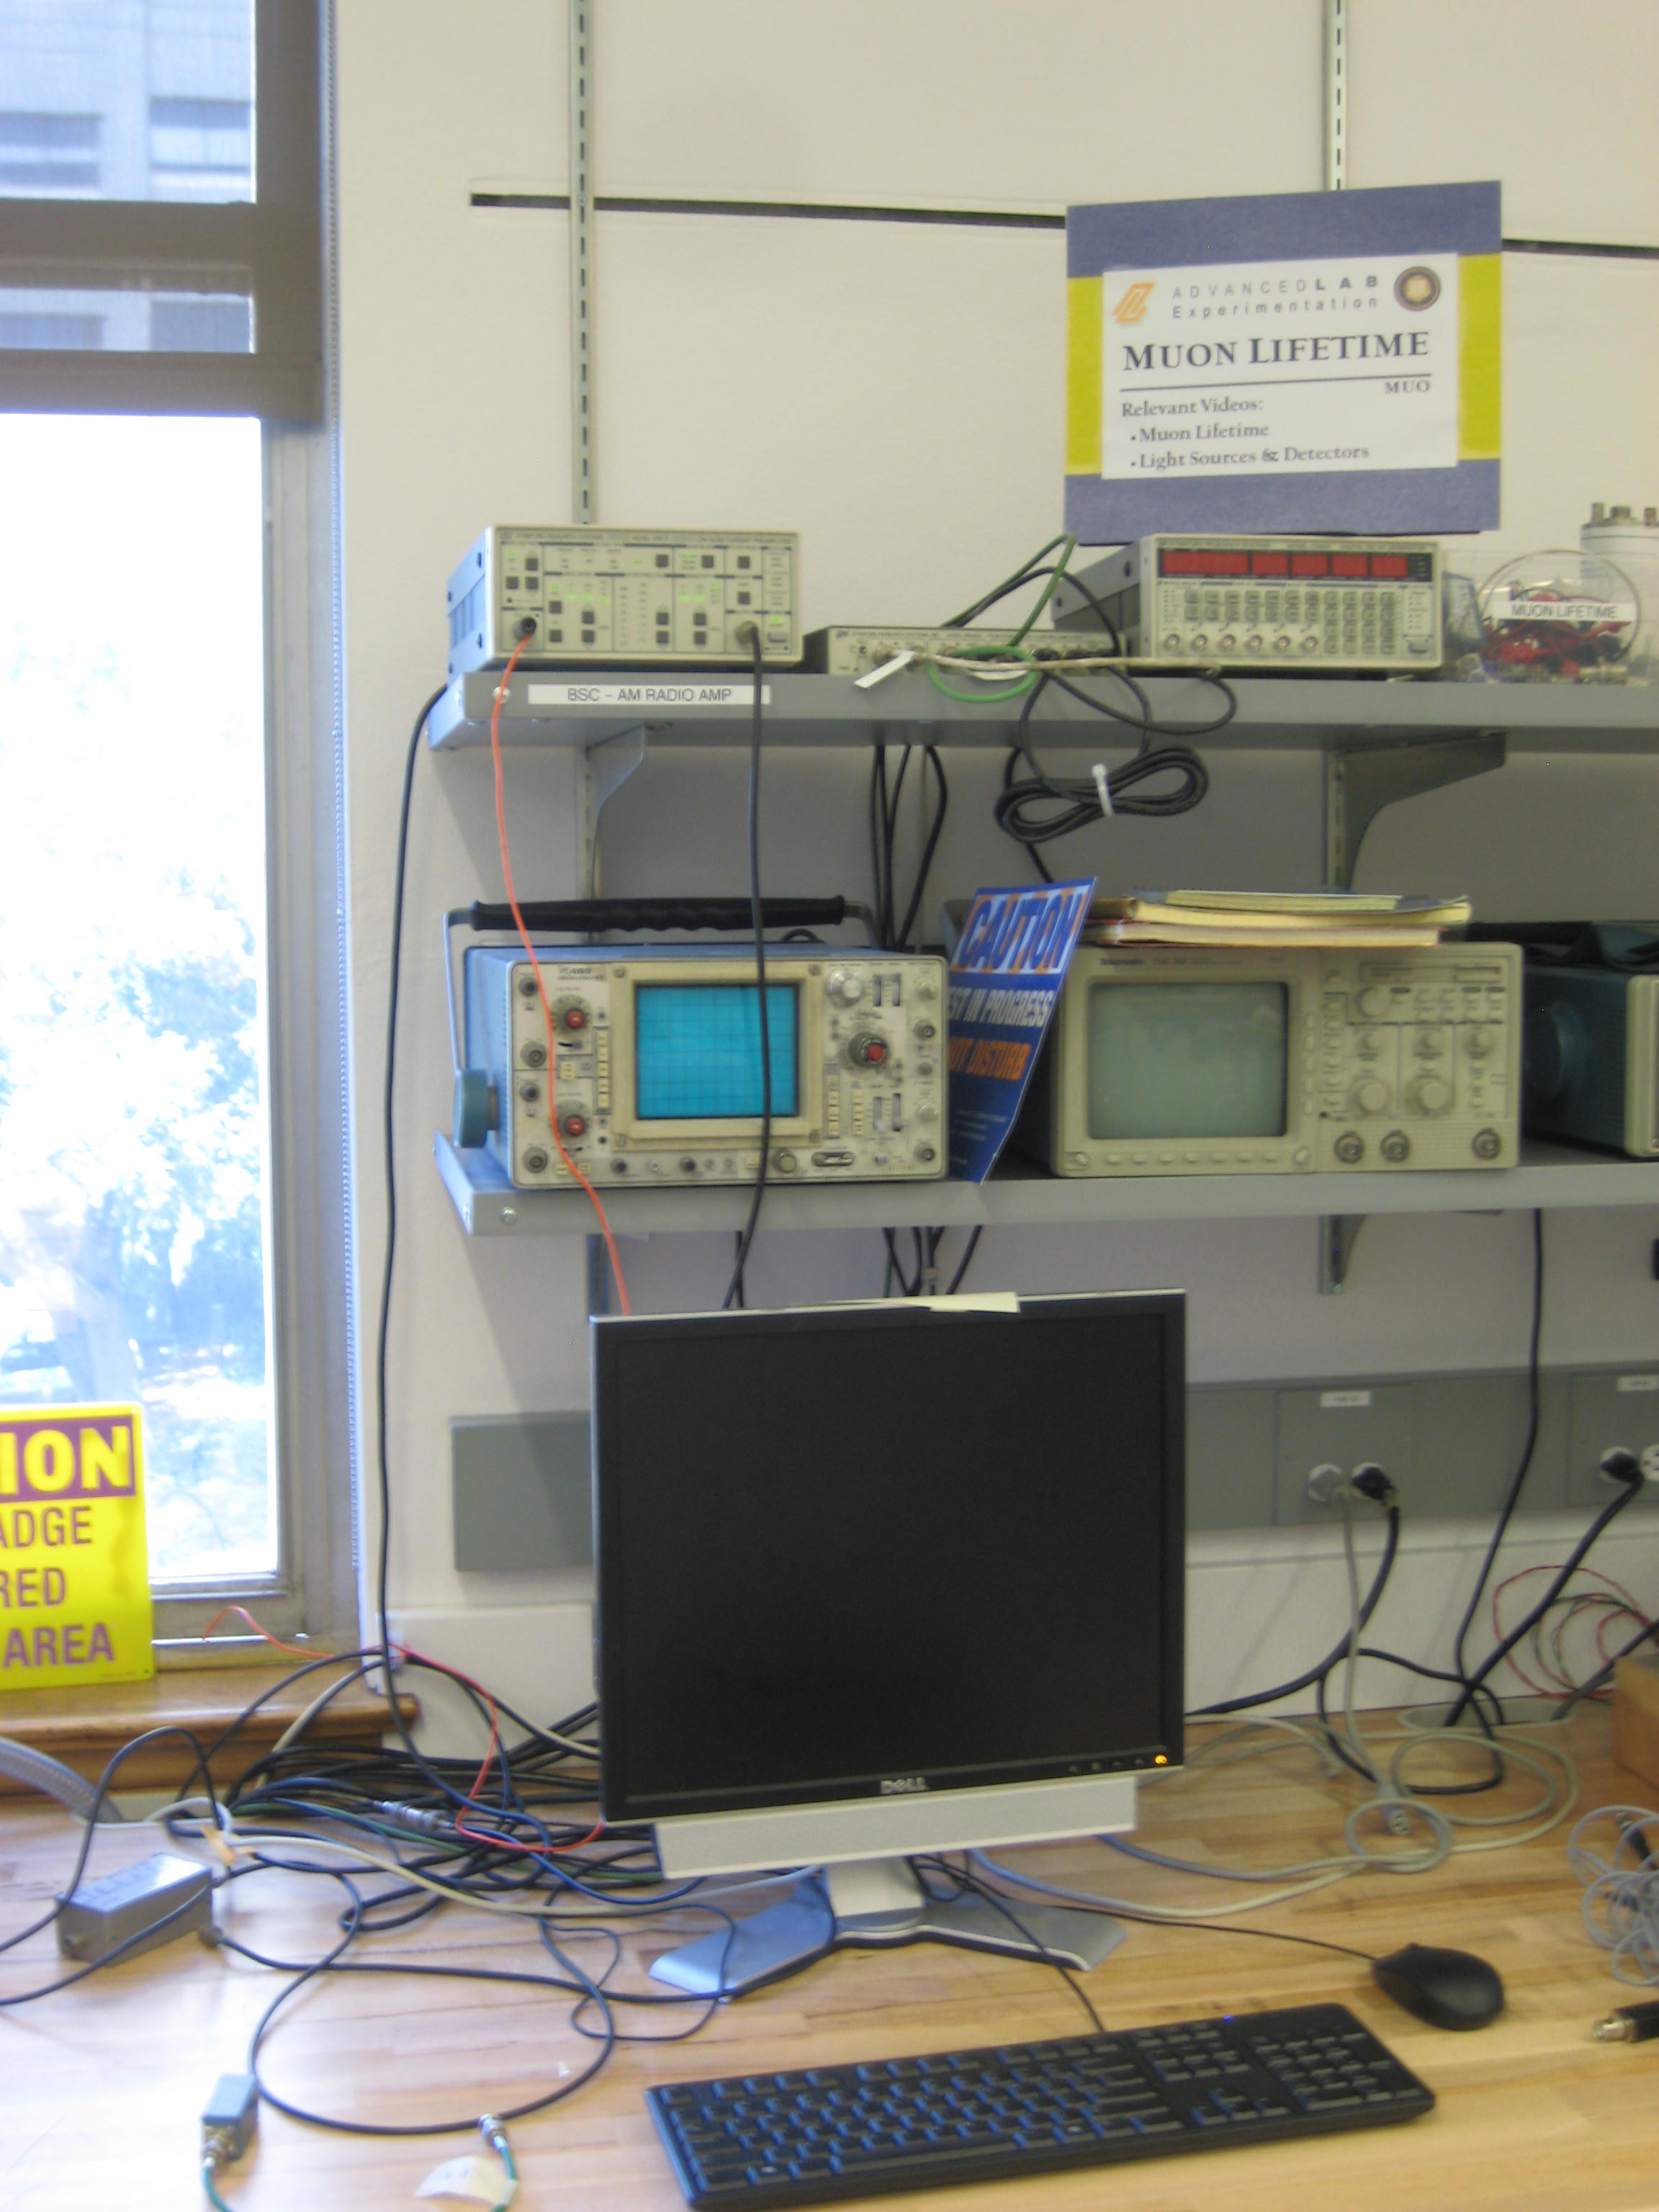
\includegraphics[width=\linewidth,keepaspectratio]{images/MUO_3517.jpg}}
    \caption{Lab station front view. See larger image \href{http://experimentationlab.berkeley.edu/sites/default/files/images/MUO_3517.jpg}{\textbf{here}}}
\end{minipage}
\begin{minipage}{0.18\textwidth}
    \href{http://experimentationlab.berkeley.edu/sites/default/files/images/MUO_Pwr_3562.jpg}{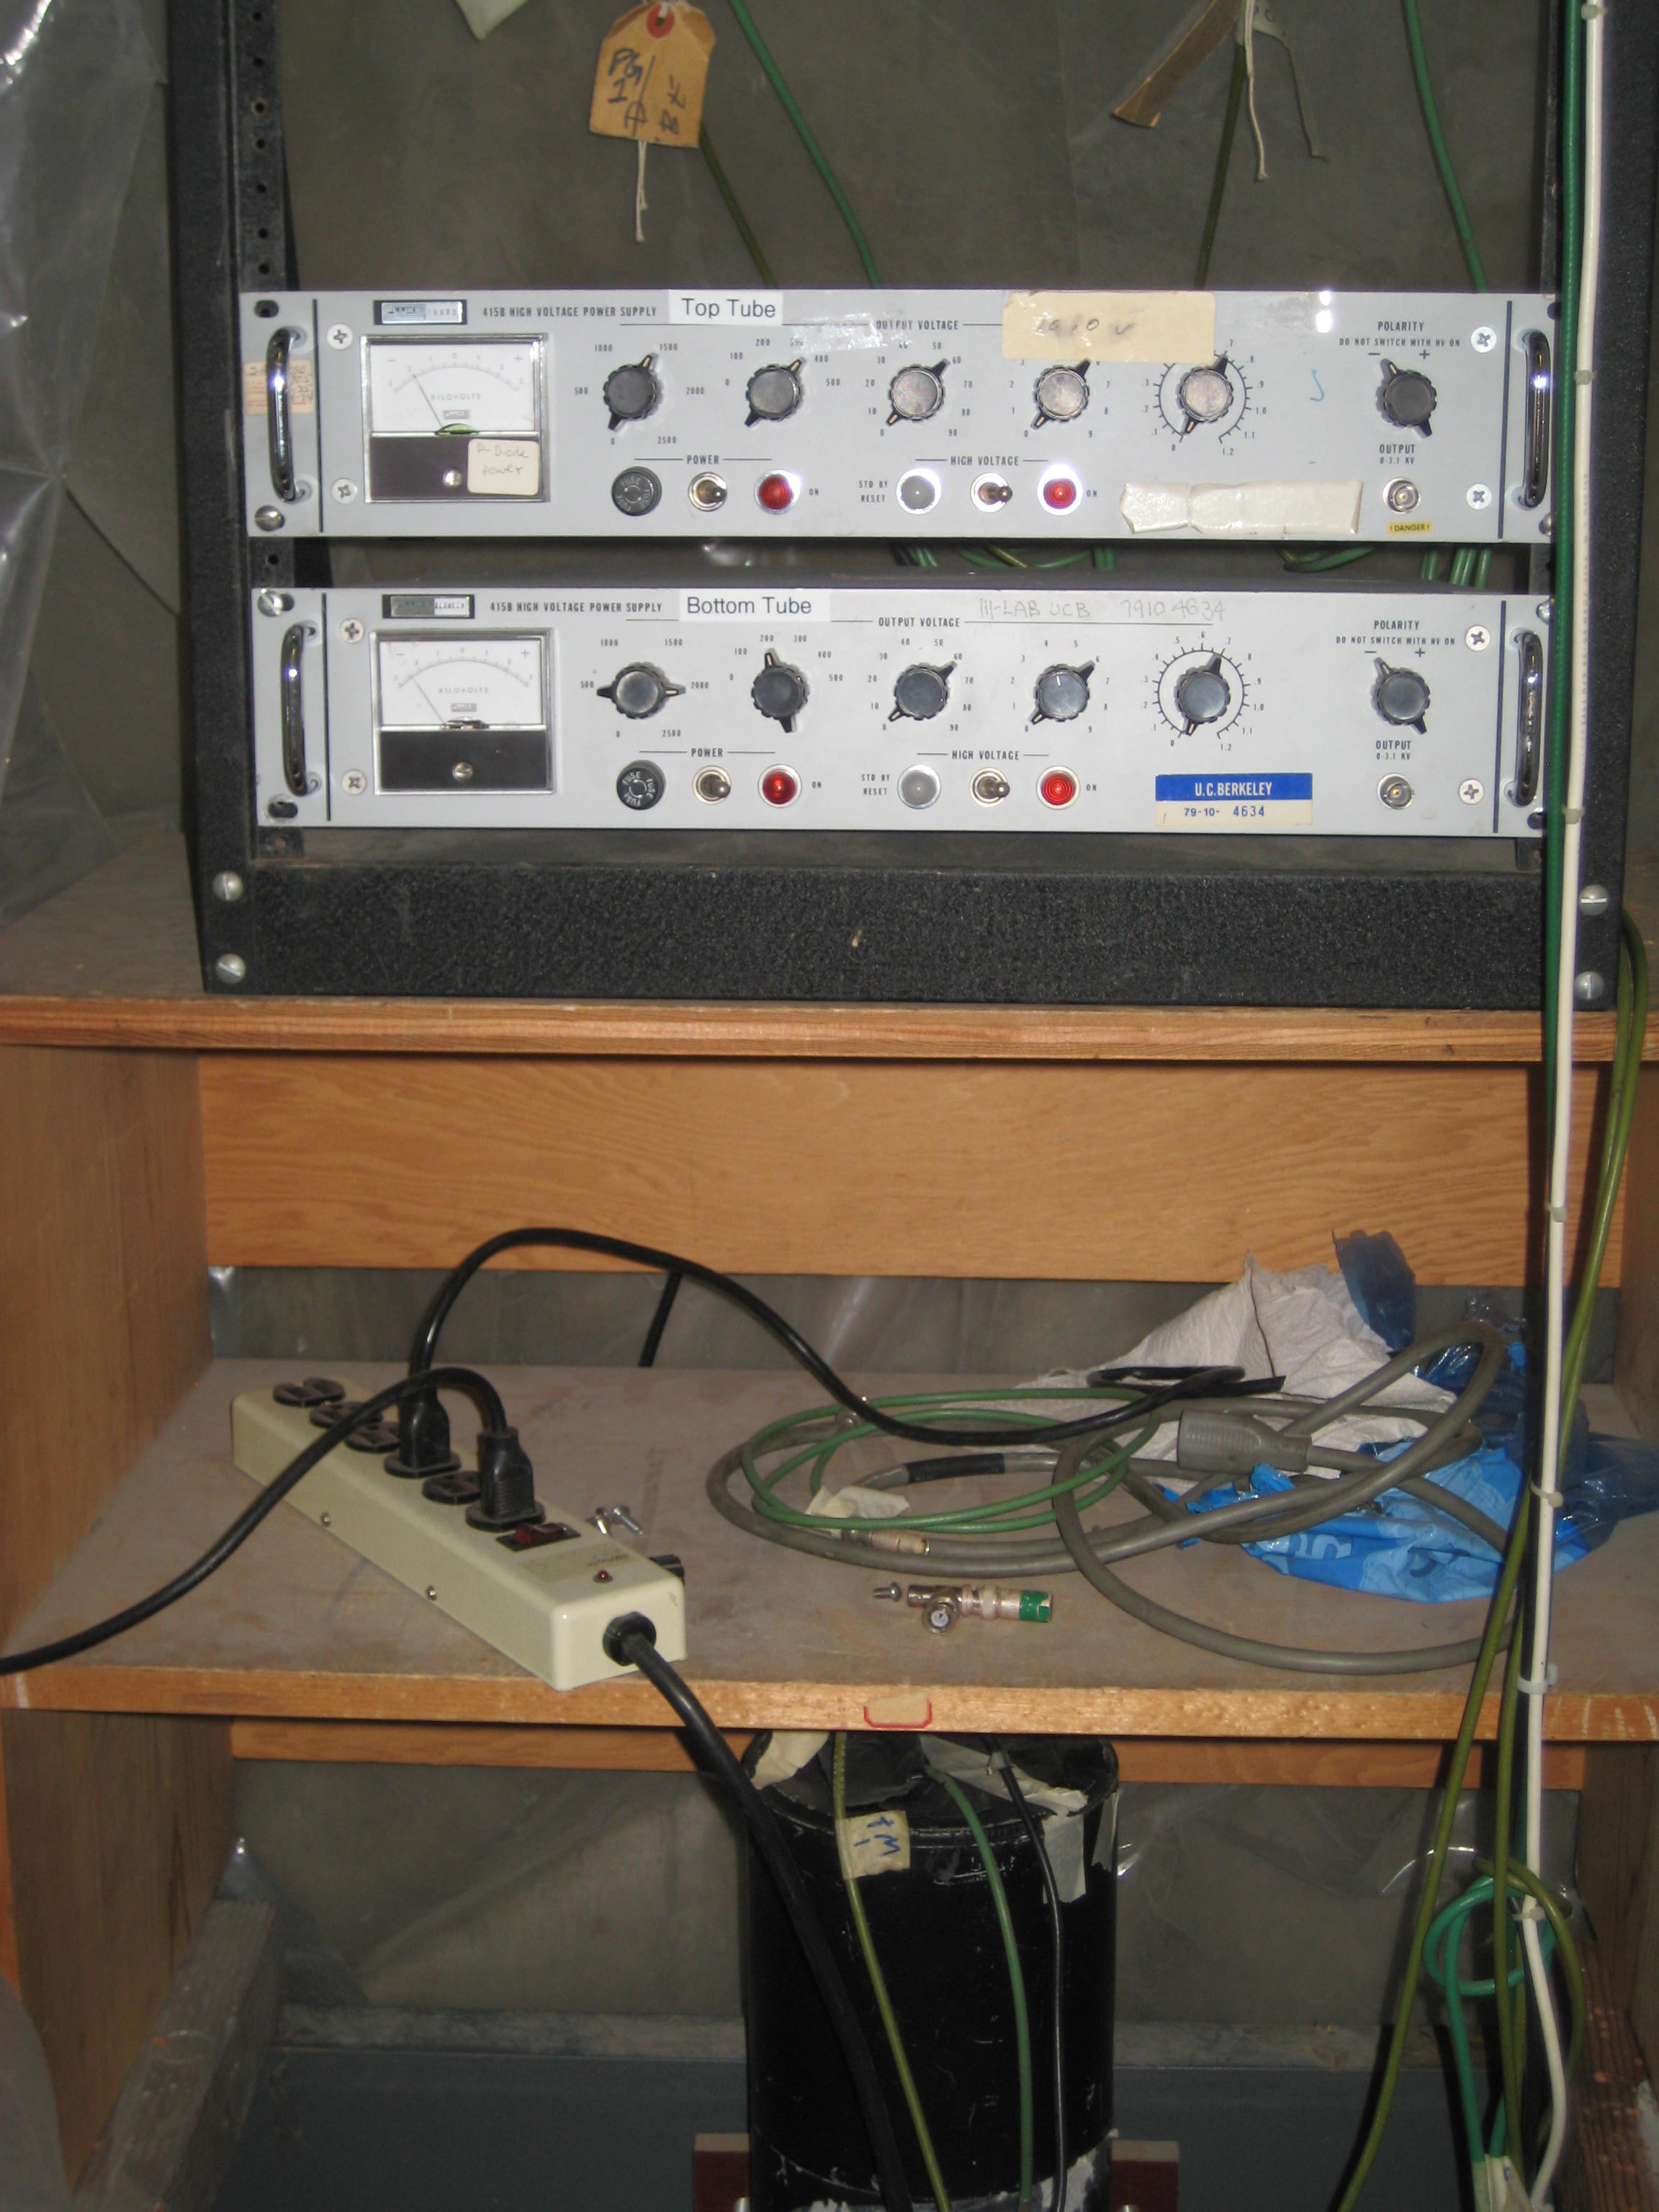
\includegraphics[width=\linewidth,keepaspectratio]{images/MUO_Pwr_3562.jpg}}
    \caption{High voltage power supplies for top \& bottom tubes with top of the top tube. See larger image \href{http://experimentationlab.berkeley.edu/sites/default/files/images/MUO_Pwr_3562.jpg}{\textbf{here}}}
\end{minipage}
\begin{minipage}{0.20\textwidth}
    \href{http://experimentationlab.berkeley.edu/sites/default/files/images/MUO_PMT_3563.jpg}{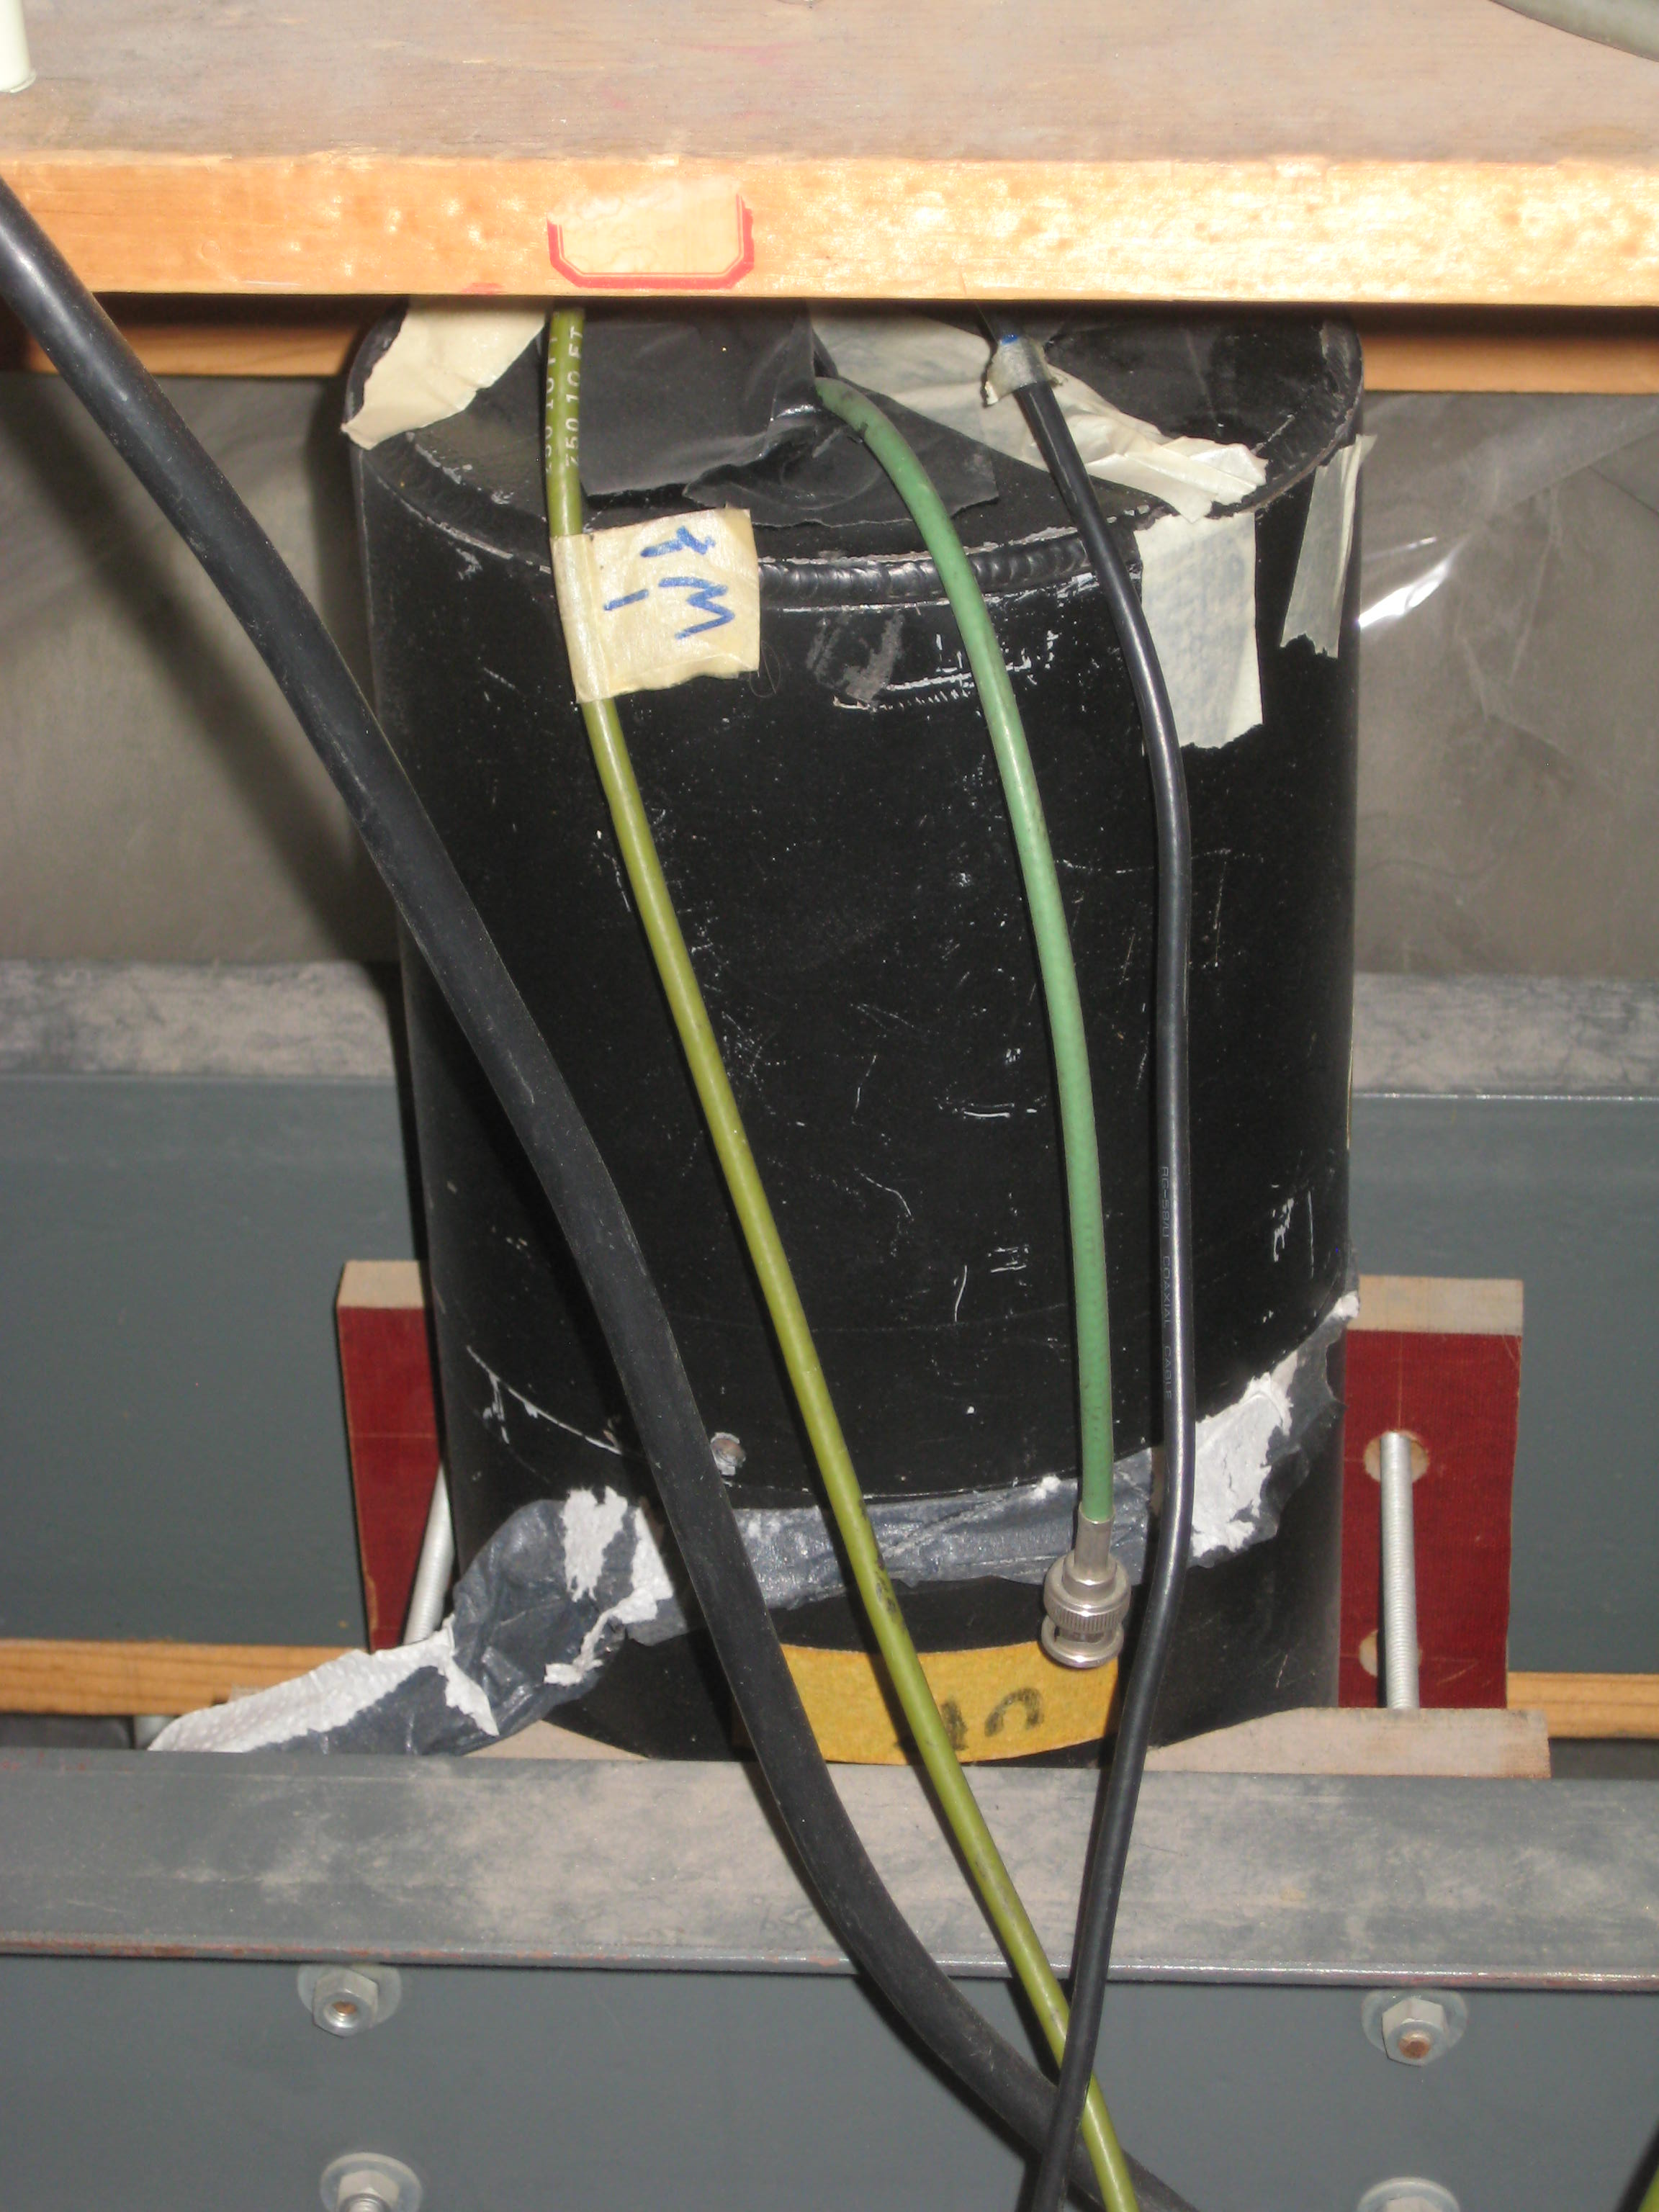
\includegraphics[width=\linewidth,keepaspectratio]{images/MUO_PMT_3563.jpg}}
    \caption{Close up of top, black photomultiplier tube found in room 275. See larger image \href{http://experimentationlab.berkeley.edu/sites/default/files/images/MUO_PMT_3563.jpg}{\textbf{here}}}
\end{minipage}
\begin{minipage}{0.33\textwidth}
    \href{http://experimentationlab.berkeley.edu/sites/default/files/images/MUO_Tank_3565.jpg}{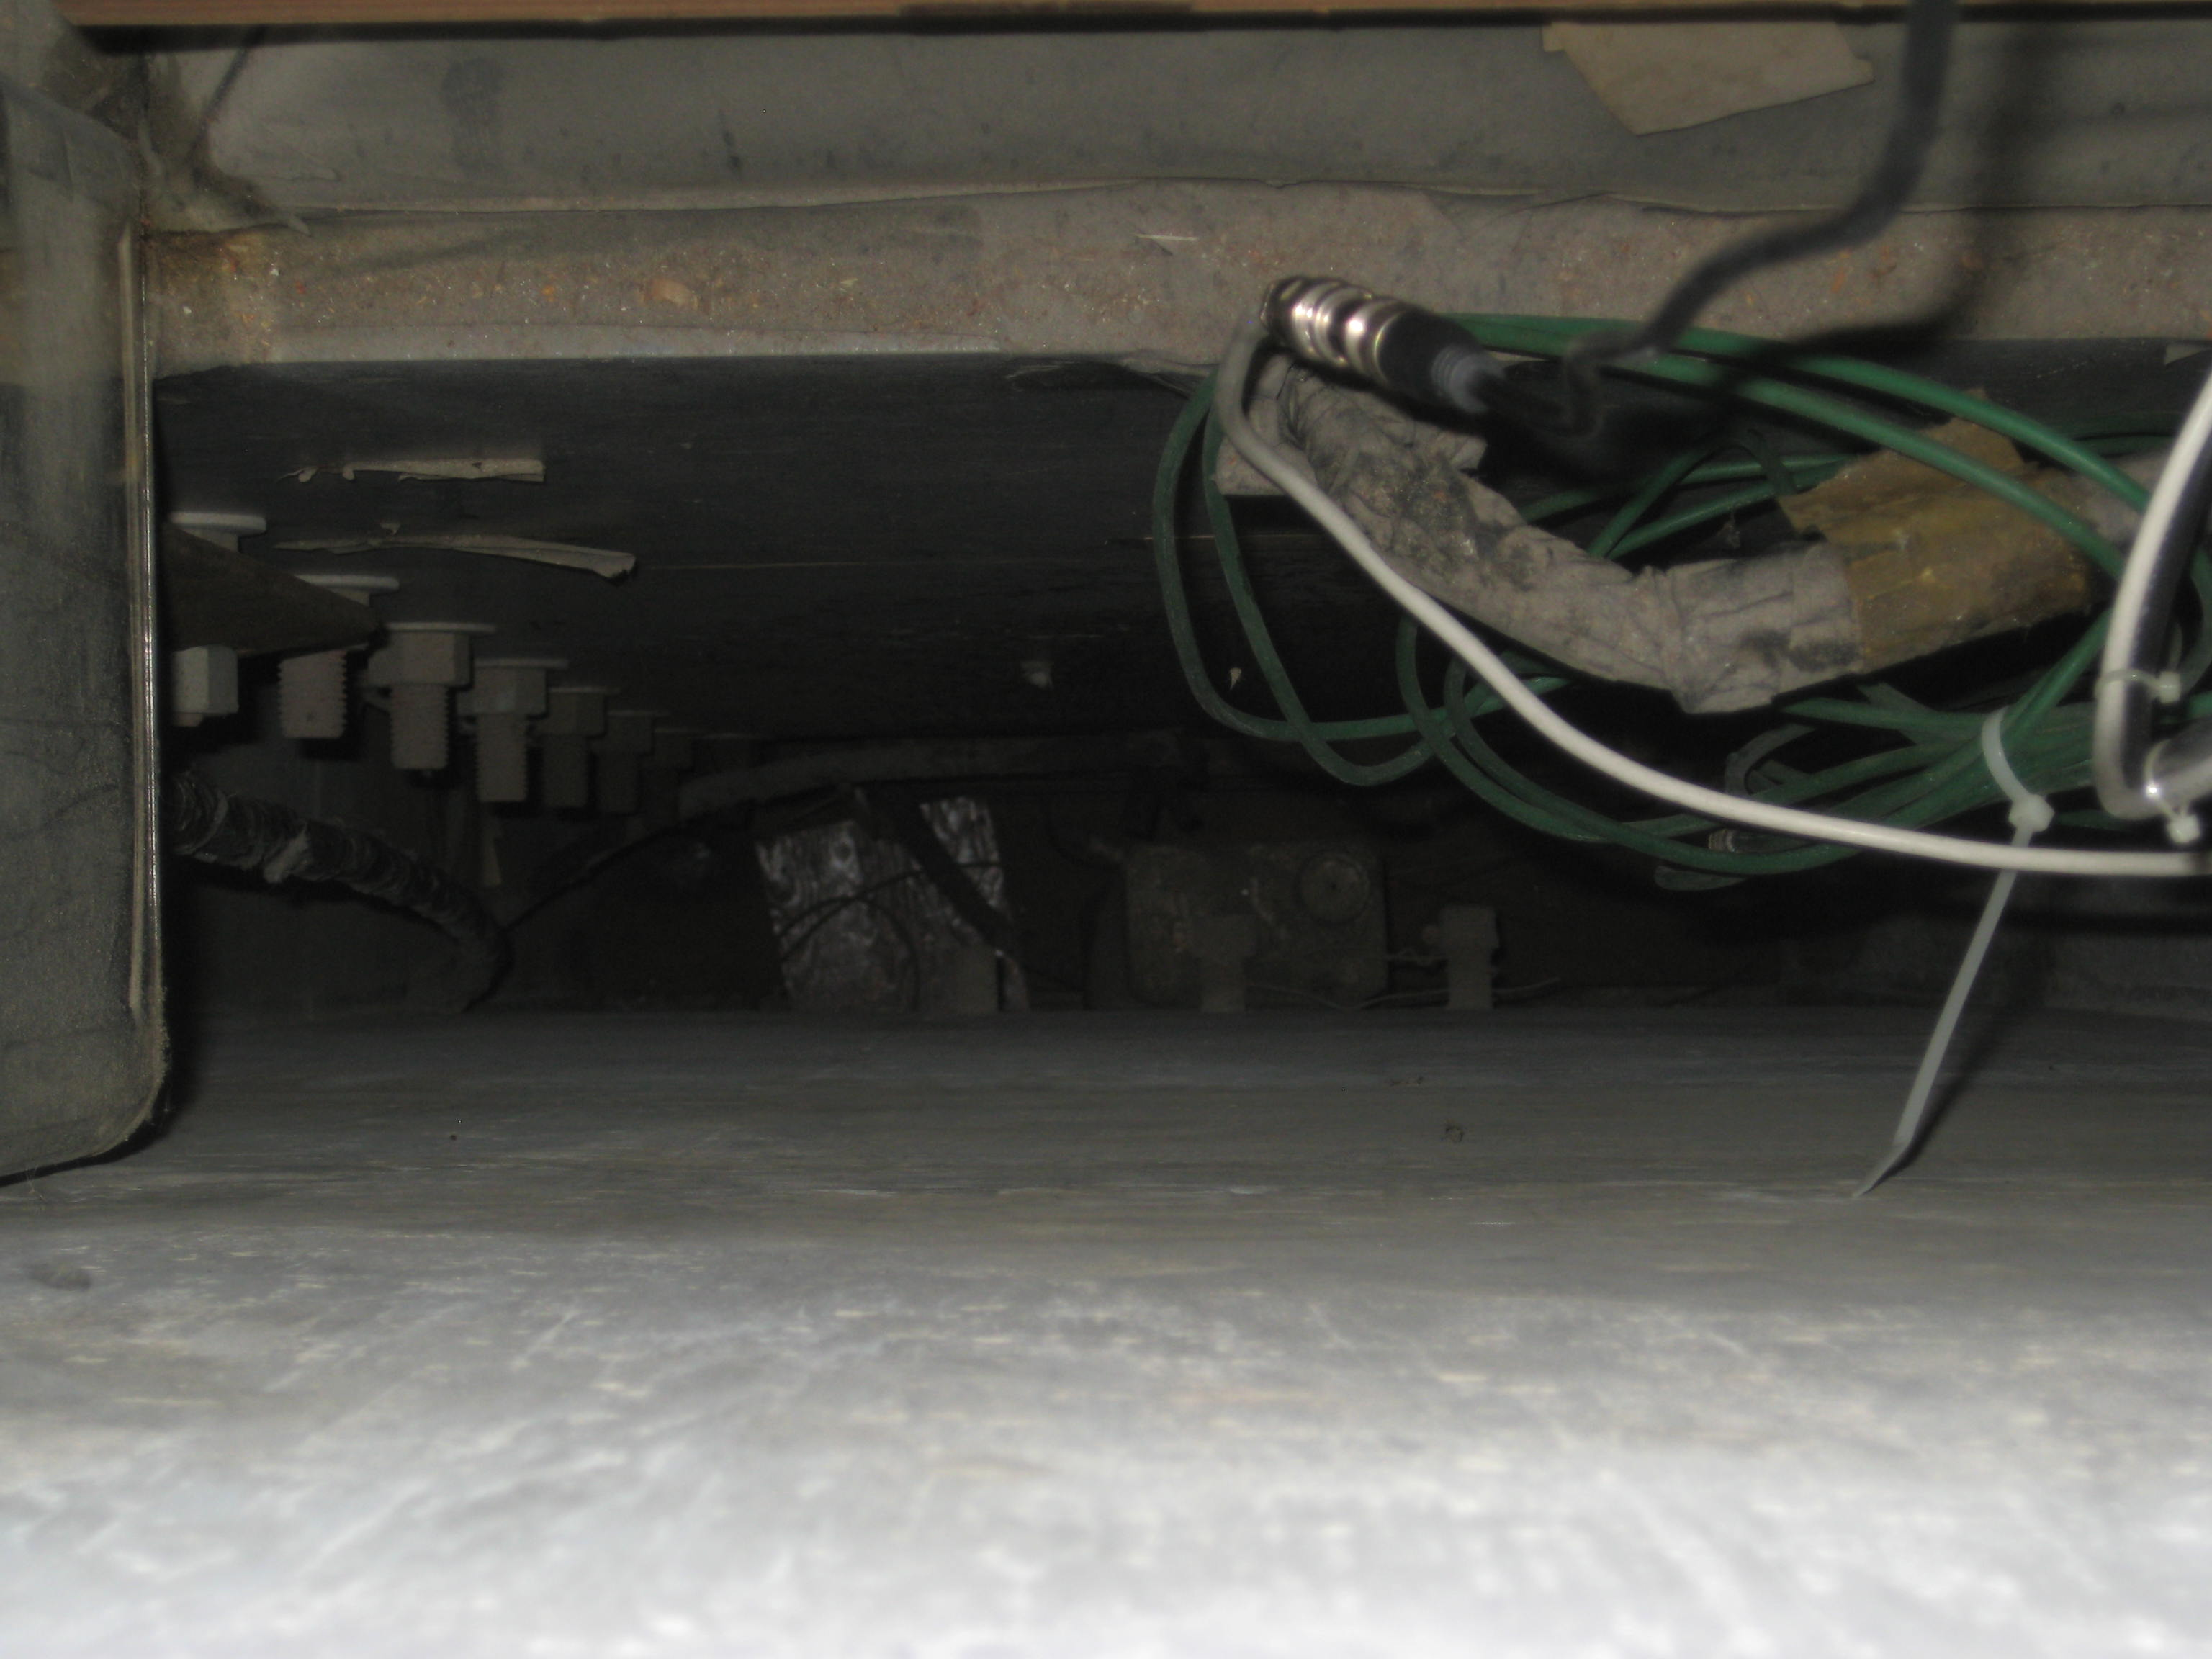
\includegraphics[width=\linewidth,keepaspectratio]{images/MUO_Tank_3565.jpg}}
    \caption{Vertical shaft found in room 275, where the large liquid scintillation tank sits. See larger image \href{http://experimentationlab.berkeley.edu/sites/default/files/images/MUO_Tank_3565.jpg}{\textbf{here}}}
\end{minipage}
\end{figure}

\newpage

\section{Before the 1st Day of Lab}

\signatures \hyperlink{Oscilloscope (TDS 360)}{ 1} \hyperlink{Apparatus in the other room}{ 2} \hyperlink{Trigger Rate}{ 3} \hyperlink{Time Difference Data}{ 4}

\begin{enumerate}
    \item \emph{\textbf{Note: In order to view the private Youtube videos hosted by the university, you must be signed into your berkeley.edu Google account.}} \\
    View the \href{http://youtu.be/uqH0qRIwBmg}{\textbf{Muon Lifetime Video}}.

    \item Last day of the experiment please fill out the \href{\ExperimentEvaluation}{\textbf{Experiment Evaluation}}

\end{enumerate}

\noindent\textbf{Suggested Reading:}

\begin{enumerate}
    \item B. Rossi, ``\href{http://rmp.aps.org/abstract/RMP/v20/i3/p537\_1}{\textbf{Interpretation of Cosmic-Ray Phenomena}}'', Rev. Mod. Phys. \textbf{20}, 537 (1948).\emph{Gives the cosmic ray flux at sea level. Figure 6 on p. 545 is important for your calculations.} \href{http://physics111.lib.berkeley.edu/Physics111/Reprints/MUO/02-Cosmic-Ray\_Phenomena.pdf}{\textbf{Searchable Page}}

    \item D. Griffiths, \emph{\href{http://physics111.lib.berkeley.edu/Physics111/Reprints/MUO/04-Introduction\_to\_Elementary\_Particles.pdf}{\textbf{Introduction to elementary particles}}}, 1987.\emph{Read the introduction (pp. 1-10). The result of a tedious calculation of the muon lifetime is given in pp. 307-309.}

    \item R.D. Evans, \emph{\href{http://physics111.lib.berkeley.edu/Physics111/Reprints/MUO/05-The\_Atomic\_Nucleus.pdf}{\textbf{The Atomic Nucleus}}}, McGraw-Hill (1955).\emph{Read about radioactive decay in Chapter 15.}

    \item C.S. Sutton et al., ``\href{http://physics111.lib.berkeley.edu/Physics111/Reprints/MUO/01-Undergraduate\_Cosmic\_Ray\_Muon\_Decay.pdf}{\textbf{Undergraduate Cosmic Ray Muon Decay Experiments with Computer Interfacing}}'', Computers in Physics, Nov/Dec, 76 (1987), \#QC52.C658.

    \item O.C. Allkofer, \emph{\href{http://physics111.lib.berkeley.edu/Physics111/Reprints/MUO/06-Introduction\_to\_Cosmic\_Radiation.pdf}{\textbf{Introduction to Cosmic Radiation}}}, Verlag Karl Thiemig, Munchen (1975). Read Sections 4.1, 9.1-9.6, 9.12, and 10.1-10.4.

    \item "\href{http://physics111.lib.berkeley.edu/Physics111/Equipment\_Manuals/RCA\_PMT.pdf}{\textbf{RCA-4522 Photomultiplier Tube Specifications}}”, RCA Electronic Components, June, 1 (1968).
\end{enumerate}

More \hyperref[sec:References]{References}

[\href{http://physics111.lib.berkeley.edu/Physics111/Reprints/MUO/MUO\_index.html}{\textbf{Physics 111 Library Site}}]

You should keep a laboratory notebook. The notebook should contain a detailed record of everything that was done and how/why it was done, as well as all of the data and analysis, also with plenty of how/why entries. This will aid you when you write your report.

\section{Objectives}

\begin{itemize}
    \item Measure Muon Lifetime

    \item Demonstrate Relativistic Time Dilation

    \item Measure Local Muon Flux

    \item Measure Sea Level Muon Charge Ratio

    \item How to Analyze a Convenient Source of Genuinely Random Numbers

    \item Create Simulate ``Muons'' and Measure their Lifetime

    \item Study Processing of Photomultiplier Signal

\end{itemize}

\section{Introduction}

The goal for this lab is to measure the lifetime of the muon. This is a relatively simple experiment, but one that can achieve surprisingly good precision if you are careful. Calibrating the electronics properly is important and is worth doing carefully. Most of the adjustments are made in the analysis using software. Don't rush through the adjustments, but ensure you understand what you are doing and how your changes affect the data. Get the settings right before spending all day and night recording data; otherwise you only find out later that the data are useless. Once you have the data and a nice plot on the screen, you still need to work hard to make a proper analytical fit and to extract a correct value for the lifetime.

Muons are particles that have a mass over 200 times that of the electron. Muon decay is of great importance in the study of weak interactions, one of the fundamental forces in nature. The value of the muon lifetime is one of the most precisely known constants, and is currently measured with a precision of a few parts per million. In this experiment, low-energy muons are primarily created from decays of particles produced in the interactions of high-energy cosmic-rays with the earth's atmosphere. Eighty percent of the cosmic rays at sea level are muons, positively or negatively charged. They have a mean lifetime of a few microseconds.

They decay by the following processes:
\begin{equation}
\label{eq:Decay1}
    \mu^-\rightarrow e^-+\bar{\nu}_e+\nu_\mu
\end{equation}
and
\begin{equation}
\label{eq:Decay2}
    \mu^+\rightarrow e^++\nu_e+\bar{\nu}_\mu
\end{equation}
By the CPT theorem, the lifetimes of the negative and positive muons in \emph{vacuum} (i.e. due to reactions \eqref{eq:Decay1} and \eqref{eq:Decay2}) are equal. However, in matter, negative muons, when brought to rest in the close neighborhood of some nucleus (Z,A) a muonic atom is formed with the muon orbiting in the K-shell. The negative muon in the muonic atom can either decay as shown in reaction \eqref{eq:Decay2}, or it can disappear through the competing reaction:
\begin{equation}
\label{eq:Reaction3}
    \mu^- + p \rightarrow \nu_{\mu}+n
\end{equation}
where $p$ annd $n$ are the proton and neutron respectively.
The rate of the muon-capture process \eqref{eq:Reaction3} depends strongly on the charge Z of the nucleus which captures the muon. In muonic carbon atoms, the rate of the muon capture \eqref{eq:Reaction3} is about 10\% the decay rate in \eqref{eq:Decay2}.

Most of the muons that are incident on the detector pass straight through it. Only the lowest energy particles come to rest within the scintillating liquid itself.

\section{Apparatus}

\subsection{Overview}

\begin{figure}[h]
    \centering
    \href{http://experimentationlab.berkeley.edu/sites/default/files/images/750px-Muon_Equip_New_fig1.png}{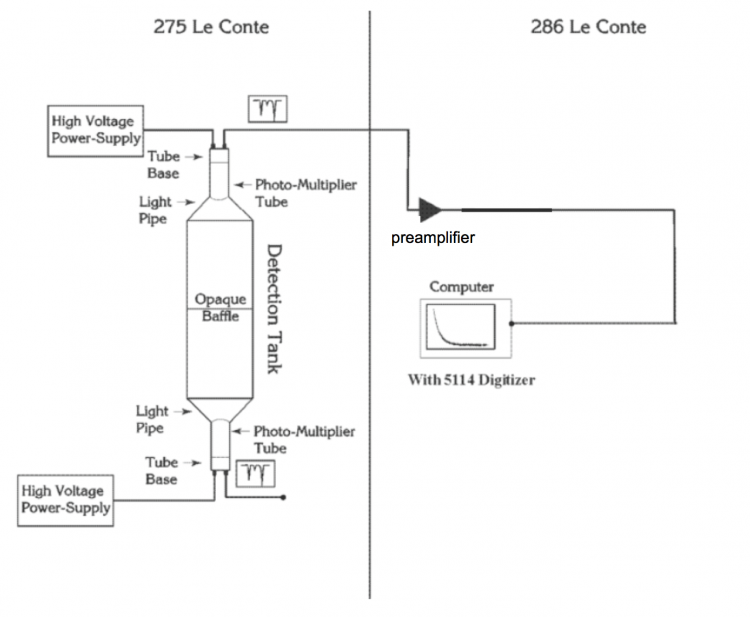
\includegraphics[width=0.5\linewidth]{images/750px-Muon_Equip_New_fig1.png}}
    \caption{Block Diagram of Muon Lifetime Experiment}
    \label{fig:BlockDiagram}
\end{figure}

The large liquid scintillation counter is located in a shaft which can be accessed from room 275 LeConte. It is filled with 125 gallons, 500 kg (1/2 cubic meter) of mineral oil in which a scintillating substance is dissolved. The passage of fast charged particles through the liquid gives rise to short pulses of light a few nanoseconds in duration. These flashes of light called scintillations are converted into electrical pulses by photomultiplier tubes located at the top and bottom of the detector (Figure \ref{fig:BlockDiagram}). Each photomultiplier views half of the tank, which is divided by an opaque baffle in the horizontal mid plane.

A photomultiplier tube (PMT) is a detector that converts single photons into large pulses of electric current by successive multiplying stages (Figure \ref{fig:PhotomultiplierTube}).

\begin{figure}[h]
    \centering
    \href{http://experimentationlab.berkeley.edu/sites/default/files/images/MUOimage056.gif}{
\includegraphics[width=0.5\linewidth]{images/MUOimage056.png}}
    \caption{Photomultiplier tube}
    \label{fig:PhotomultiplierTube}
\end{figure}

\noindent\textbf{In the shaft of room 275 LeConte Hall} (Get a GSI to let you into the room) \textbf{are located:}

\newpage

\begin{itemize}
    \item a high voltage supply and a high voltage divider for the photomultiplier tubes. The high voltage of the photomultiplier tube normally is left on and is NOT adjusted by the student. See the staff in the 111-LAB. These photomultiplier tubes are irreplaceable. Do not mess with them.

    \item a voltage meter to read the individual high voltages. \emph{\textbf{Under no circumstances should the high voltage exceed 2200 V!}}

    \item one large liquid scintillator with 500 kg of doped mineral oil

    \item cables leading to 286 LeConte where the rest of the apparatus is located.
\end{itemize}

\noindent\textbf{At the 286 LeConte Muon Lifetime Station are located:}

\begin{itemize}
    \item SR445A 4-channel x5 amplifier, for amplifying the signals from the top PMT (white cable) and bottom PMT (black cable). The flashing red lights should indicate that they are receiving a signal.

    \item Tektronix TDS 360; Digital Storage Scope

    \item Tektronix 465 Oscilloscope (Analog)

    \item Miscellaneous equipment for calibration of the system and 50 ohm terminators

    \item Stanford Research Systems Model DG645 Digital Delay Generator

    \item National Instruments Digitizing Card \# NI-5114

\end{itemize}

\noindent This Digitizer works together with a LabVIEW program that does two things: (1) it is an oscilloscope, (2) it is a differential detector logic system.

\subsection{How the Experiment Works}

\newpage

Muons are derived from the process of cosmic ray particles striking the nuclei of atoms and molecules in the atmosphere. A muon that passes through the liquid scintillator tank generates scintillation. A photomultiplier tube picks up the light pulse and sends an electrical signal through a cable to our experiment. A muon that enters, stops, and subsequently decays in the liquid scintillator gives rise to two pulses separated by a few microseconds, one when it enters the liquid, and a second one when it decays. The pulses can be viewed with an oscilloscope or digitized and stored on the computer. You are going to measure the time difference between these correlated pulses, as well as the amplitude and width of each pulse. After many such observations, you will obtain a distribution of the number of counts vs. time difference. Ideally, when these data are plotted, they will form an exponential decay curve, whose decay constant is the lifetime of the the muon.

\begin{figure}[h]
    \centering
    \href{http://experimentationlab.berkeley.edu/sites/default/files/images/MUOimage008.gif}{
\includegraphics[width=0.5\linewidth]{images/MUOimage008.png}}
    \caption{This graph shows lifetime on the X axis and counts on the Y axis. Note that the X axis  sometimes is called the channel number for the digitizer. The Y axis is also called the amplitude counts.}
    \label{fig:MUOimage008}
\end{figure}

When the two pulses come down the cable, they are routed to an amplifier. Then they go to the National Instruments Digitizer Card NI 5114. You configure triggering and timing properties of the digitizer in the LabVIEW programs. The LabVIEW program \textbf{Muon Detection Program} coupled to the digitizer card detects pulses from two photomultiplier tubes, measures their arrival times, amplitudes, and widths, and, for a subset of pulses that satisfy a preset criteria, writes the data to disk. You will read the data offline, filter it to reject noise, plot the time difference between two pulses in the same photomultiplier tube, and use the distribution to measure the muon lifetime.

\subsection{Explanation of the LabVIEW Programs}

\href{http://experimentationlab.berkeley.edu/sites/default/files/Muon/Viewsignalsprogram.png}{\textbf{Screenshot of the View Signals Program}}

\noindent\href{http://experimentationlab.berkeley.edu/sites/default/files/Muon/MUONdetectionprogram\_2.png}{\textbf{Screenshot of the Muon Detection Program}}

\newpage

\checkpoint{Oscilloscope (TDS 360)}{Before you use these programs you should have viewed the signals with a real oscilloscope (TDS 360). What polarity are they, positive or negative? How wide, how high, etc. The TDS 360 will trigger depending upon the polarity of the signal, it is important to understand what polarity the signals are before moving on to the LabVIEW program as it will need to be specified when the data acquisition begins. The trigger level on the lab view program is initialized to some arbitrary voltage, however this is not the correct voltage that is capable of reading both the peaks coming from the PMT and filtering out the low voltage noise. Therefore the purpose of hooking the signals up to the oscilloscope is to get a visual reading and estimate of the heights in voltage space and separation between the initial interaction peak and the decay peak in time (your brain and eyes make a great team in pattern recognition). Warning: You do not want to trigger on too low of a voltage, the erratic spread of oscillations are simply noise and you are looking for very narrow sharp peaks following the initial large decaying spike. Show GSI your pulse signals on the oscilloscope and discuss what values you think are appropriate for the LABView program.}

%\textbf{This is a Checkpoint: Before you use these programs you should have viewed the signals with a real oscilloscope (TDS 360). What polarity are they, positive or negative? How wide, how high, etc. The TDS 360 will trigger depending upon the polarity of the signal, it is important to understand what polarity the signals are before moving on to the LabVIEW program as it will need to be specified when the data acquisition begins. The trigger level on the lab view program is initialized to some arbitrary voltage, however this is not the correct voltage that is capable of reading both the peaks coming from the PMT and filtering out the low voltage noise. Therefore the purpose of hooking the signals up to the oscilloscope is to get a visual reading and estimate of the heights in voltage space and separation between the initial interaction peak and the decay peak in time (your brain and eyes make a great team in pattern recognition). Warning: You do not want to trigger on too low of a voltage, the erratic spread of oscillations are simply noise and you are looking for very narrow sharp peaks following the initial large decaying spike. Show  GSI your pulse signals on the oscilloscope and discuss what values you think are appropriate for the LABView program. }
\begin{itemize}
    \item Note: High voltage on the PMTs are as follows, Top tube =1900 Volts Negative and bottom tube = 2300 Volts Negative with the SR445A 4 each amplifier, setup top PMT 1 -amp, bottom PMT 2 amps.

\end{itemize}

This experiment uses two different LabVIEW programs: \textbf{View Signals} and \textbf{Muon Detection Program}. The purpose of \textbf{View Signals} is for you to choose the best input parameters by inspecting the signals and seeing how changes in the input parameters affect the signals and counting rates. (This reads the input signals like an oscilloscope). The optimal input parameters should then be used in the program \textbf{Muon Detection Program}, whose purpose is to save pulses to data files, from which you calculate the muon lifetime.

\newpage

A high-speed digitizer installed in the back of the computer receives two signals. The digitizer represents the incoming analog signal by generating a series of numbers that describes the discrete samples. The top PMT is connected to Channel 0 of the digitizer, and the bottom PMT is read out by Channel 1. The digitizer is configured and initialized when you click \textbf{Start Acquisition} in either of the Muon LabVIEW programs and essentially a programmed way to interpret the incoming signal. However since the digitizers purpose is to represent the incoming signal and process the data you can change its configuration throughout the program. You can set the input range for each channel separately; 2 V is about right for both channels (the offset is set to 20\% of the range, so 2V corresponds to the range [$-$0.4V..+1.6V]). The input impedance is set to 50 ohms and the digitizer uses full bandwidth.

Here is a brief description of the different program controls (a more detailed explanation is given in the following section):

The user control \textbf{Range (microseconds)} determines the minimum length of the record (counting from the trigger), i.e. the maximum difference between the trigger and the second pulse. The triggering event is set to be at 12\% of the way through each record, so that the digitizer can see pulses just before the trigger. The user control \textbf{Min sample rate} specifies the minimum sample rate (leave it at 250 MHz). The type of triggering is set to analog edge triggering. You can select to trigger on Channel 0, Channel 1, or External (which we do not use). The trigger slope is set by the user control \textbf{Pulse polarity}, and the user control \textbf{Trigger level} sets the trigger level. For signals with negative polarity you want to make sure that the green light is on and the signal is flipped, you can determine the polarity of the signals by hooking them up to the oscilloscope.

Both programs initiate a record acquisition by the digitizer and, once the voltage exceeds the trigger threshold, retrieve voltage waveform data for both channels, incrementing the \textbf{Trigger Count} by one. The programs remove the voltage offset by averaging the voltages of the first 200 samples of the record, all of which should occur before the triggering event, and subtracting that voltage from all the voltage waveform data. The programs then search for up to two pulses below (for negative \textbf{Pulse polarity}) or above (for positive \textbf{Pulse polarity}) the \textbf{Channel 0(1) threshold,} which you set. This threshold is relative to the offset, not ground. The first pulse will correspond to the Muon entering the scintillating material within the tank and the second to its decay. The time difference between the first and second pulses has to be less than the \textbf{Range}, which you set, and greater than the \textbf{Pulse 2 delay,} which you set. The range is simply a measure of how long the program will wait between pulses before moving on to the next signal. The pulse 2 delay is there in order to ignore any noise generated after the first signal that may pass the trigger level. Typically 1 microsecond is enough breathing time. You can specify how many pulses in each channel is required for the data to be written to disk, for our case we are looking for two events (i.e. the incident and the decay). The \textbf{Output Count} is incremented if exactly that number is found in each channel. Whether or not the output condition is satisfied, the process repeats with the next data record.

It is important to note that in the program \textbf{View Signals}, after clicking \textbf{Start Acquisition}, the program continues to acquire records from the amplifier and searches them for the specified pulses until you click \textbf{Stop Acquisition}. This program graphs the \textbf{Raw signals} acquired by the digitizer, the \textbf{Signal with offset removed} and the \textbf{Filtered signal} -- for each channel (Channel 0 in white, Channel 1 in red).

Once you have determined the optimal settings for the program controls the next portion of the lab deals with the\textbf{ Muon Detection Program }which measures the pulse height and width in addition to time. To reduce noise, the programs pass the waveforms through a 29-tap low-pass filter. You set the cut-off frequency of the filter with the control \textbf{Lower-cut off frequency}. \textbf{Pulse 1 threshold} and \textbf{Pulse 2 threshold} correspond to the unfiltered signal. Unfiltered pulses that meet these thresholds will have their amplitudes reduced upon filtering.

\newpage

When you click \textbf{Start Acquisition}, the program prompts you to enter two different file paths to save data: a temporary local data file and a network data file. The temporary file is supposed to be on local disk (``C:/'') so that network connectivity does not affect performance. The temporary file is copied to the network storage (your ``Documents/'' directory) when the program terminates. After the files are open, the program begins acquiring records and searching them for pulses. When an output condition is satisfied (i.e. exactly the specified number of pulses is found in each channel, up to the maximum of 2), the program writes out a record of 12 floating-point numbers to the temporary file: time, amplitude, and width of four pulses: 1st pulse in Channel 0, 2nd pulse in Channel 0, 1st pulse in Channel 1, 2nd pulse in Channel 1. If a given pulse is not found in the record, the time, amplitude, and width are assigned zero values. \textbf{IMPORTANT FOR DATA ANALYSIS:} It is the values saved in this text file that you will be working with in the analysis of this lab. This is the file that you should be uploading to MatLab or ROOT as it will have all the information about the signals received from the PMT.

As the program runs, it updates a histogram of decay events, where the x-axis specifies the time between the two registered pulses. If everything is working correctly, this should mimic the Muon lifetime decay curve.

The program measures the amplitude and the full-width-half-max of each peak from the signal out of the filter. The filter removes a lot of the noise, so the amplitude and width information are more accurately measured with a filter. Timing information is more accurately measured before the signal is filtered.

\subsubsection{Program Controls}

\textbf{Flip polarity}

In order for the program to run successfully, a positive signal with respect to ground is expected on both channels. However, the incoming signal from the experiment may be negative, which would crash the program. Enabling \textbf{Flip Polarity} negates the incoming signal, so that a negative signal becomes positive. If the incoming signal is already positive, \textbf{Flip Polarity} should be disabled.

\textbf{Select Trigger}

This control is identical to selecting a trigger channel on an oscilloscope. When a large enough pulse (see \textbf{Trigger Level}) is seen on the selected channel, the program collects data on both channels for a time duration set by \textbf{Range}, and then processes those signals for peaks.

\textbf{Trigger Level (V)}

This defines the signal amplitude which is required for the trigger to be activated.

\textbf{Pulse Detection Threshold (V)}

Once the trigger is activated, the program scans the collected signal for pulses. This control defines the minimum amplitude of a signal in order for it to be recognized as a pulse. Any part of the signal which is above this threshold will be recognized as a pulse, and any part which is below this threshold will not be recognized as a pulse.

\textbf{Pulse 2 Delay (μs)}

Once the trigger is activated, we wish to ignore any pulses that occur shortly after, since they may simply be noise, as opposed to a muon decay event. This control allows the user to define how long this ignore period should last. This control should be large enough to ignore this noise, but not so large as to ignore a significant portion of the actual muon decay events.

\textbf{Range (μs)}

After the trigger is activated, the program must collect the signal which is to be analyzed for some amount of time. This control allows us to set that time duration. After this time has passed, the program analyzes the collected data for pulses, and then returns to listening for the next trigger event. This control should be just large enough to encompass a large majority of decay events.

\textbf{Exact Number of Pulses}

Once the program has identified all of the peaks existing on the most recently received signal, it must determine whether or not these pulses represent a muon decay event. The event is registered as a true muon decay event only if the number of pulses on Channel 0 and on Channel 1 match exactly with the specified \textbf{Exact Number of Pulses}. There are three suggested use cases: [CH0 = 2, CH1 = 0]: This signifies a muon which entered the chamber connected to channel 0, and then decayed in that same chamber at a time at least as long as defined by \textbf{Pulse 2 delay}, but no longer than \textbf{Range}. Since there are only two pulses on this channel and no pulses on the other channel, we are convinced that another muon did not interfere with the measurement. For this setting, the user should set the trigger on Channel 0. [CH0 = 0, CH1 = 2]: Same as above, only for the chamber connected to channel 1. For this case, the user should set the trigger on Channel 1. [CH0 = 1, CH1 = 1]: This represents a muon event in which a muon is first detected in one chamber, but then its decay is detected in another chamber, and no other pulses are recorded. It is suggested that for this case, the trigger Channel is set to the Channel which is connected to the chamber which is on top, since more likely than not, we expect the muon to come from the above the surface of the Earth, and not below.

\textbf{Vertical Range}

This control allows the user to define the vertical range of the digitizer channel. This is analogous to setting the vertical range of a channel on a regular oscilloscope. This value should be just large enough to encompass the amplitude of any received pulse.

\textbf{Low Pass Filter Cutoff}

The program passes a received signal through a Low Pass filter, in order to reduce noise. This sets the cutoff for that filter.

\textbf{Min Sample Rate}

This parameter sets the sample rate of the digitizer.

\section{Procedure}

\subsection{Inspecting the apparatus and the signal}\label{sec:Inspect}

\begin{enumerate}
    \item Inspect the apparatus in 275 LeConte: (Get GSI to let you into the room.)

    \begin{itemize}
        \item Check the voltage setting of the PMTs but do not change (the knobs on the power supply are accurate, not the power supply's meter).

        \item Notice the color of the co-axial cables going to 275 LeConte.

    \end{itemize}

    \item Return to the apparatus in 286 LeConte:

    \begin{itemize}
        \item The cables that originate in 275 LeConte should be connected to the amplifier. Check the gain setting of the amplifier. The preamp is set for a x5 gain for both the top PMT (white cable) and x5 for the bottom PMT (black cable).

        \item Using a fast digital storage oscilloscope (Tektronix TDS-360), observe the output of the amplifiers. The cable must be terminated at the oscilloscope with a 50$\Omega$ (what happens if it is not? Try it).

        \item The scope should be set on the fastest sweep, high sensitivity ($\sim$0.2 V/div), and high beam-intensity, and triggered internally with a threshold just short of ``free run.''

        \item You should see pulses at $\sim$100-1000 Hz up to $\sim$1.0 volt in amplitude, followed occasionally ($\sim$1 Hz rate) by smaller delayed pulses. Many of these are muon decays, others are the result of various sources of noise. This is where the evolutionary capabilities of your eyes and brain working together will come in handy! Look for sharp peaks and note where they are in $x$ and $y$ space.

        \item Note the polarity, typical magnitude, and width of the pulses

        \item Once you have all this information written down it will make optimizing the LabVIEW program a lot easier.

    \end{itemize}

\end{enumerate}

\checkpoint{Apparatus in the other room}{Make sure you have seen the apparatus in the other room. Explain why the cable is terminated at the oscilloscope.}

%\textbf{ This is a Checkpoint: Make sure you have seen the apparatus in the other room. Explain why the cable is terminated at the oscilloscope. }

\subsection{Determine optimal settings using the LabVIEW program View Signals}

\textbf{Program operation and description} \href{http://experimentationlab.berkeley.edu/node/88}{\textbf{National Instruments Digitizer VI}}

\begin{enumerate}
    \item Now use the LabView Program \textbf{View Signals} on the desktop.

    \begin{itemize}
        \item If the pulses coming into the digitzer card are negative, \textbf{Flip Polarity} should be enabled.

        \item Estimate the average height of the primary and delayed pulses.

    \end{itemize}

    \item Inspect the amplified pulses with ViewSignals VI. Vary the frequency cutoff and observe how the signal and noise change. Pick the frequency cutoff that optimizes signal/noise ratio. Set the thresholds so that the counting rates (both input and output) make sense. Both should be safely above the noise level.

    \begin{itemize}
        \item For the standard data taking (i.e. when you will be collecting data for measuring the muon lifetime), you will require 2 pulses in the top PMT (Channel 0) and 0 pulses in the bottom PMT (Channel 1). What does this setting mean?

    \end{itemize}

    \item You will use the pulse generator (SRS DG645) to simulate a sequence of two pulses of approximately the size and width as the output of the detector in Room 275 LeConte later for calibration. Thus, you should get familiar with using the pulse generator. The first thing you should take note of is the front panel of the SRS DG645 for producing the pulses. The ''edge'' section is located on the left side of the display. The ''edge'' refers to the 5 different output channels, each with a 50 ohm impedance, located in the bottom of the front panel under the display. You will notice that the outputs have two letters associated with them, each located on a different edge of the signal. The first edge refers to the offset above ground and the second edge to the step size, this will effectively determine the peak-to-peak voltage of your signal above ground (an example would be A and B, where A is the offset and B is the step size). Under the display there is a section labeled ``display'' where you can navigate the different edges and move the cursor on the display (indicated by the character that is flashing). The two signals should be connected to ports AB and CD. Adjust the voltage for the expected peak heights as discovered in Section \ref{sec:Inspect} (``inspecting the apparatus and the signal''). Next you will want to set the delay of the second pulse relative to the first. This can be accomplished by pushing the ``delay'' button located in the display section. It will prompt you to input a time delay in seconds, notice the white lines and labels located right above the display, these provide you with the units of input for your delay. Simply move the cursor over to the digit you wish to change and then adjust using the up and down arrows located directly under the ‘MODIFY” section. However, make sure that when you set the delay you are selecting the correct edge to delay and that the green LED light is on for the output programmed to be the second pulse (for example if you want CD to have a delay you would make sure the LED green light is located on C and adjust the delay time). The width of the pulse can also be determined by the delay function, however now the delay is not between different outputs, but rather it is between different edges of the same output. Make sure that the LED green light is located on the second edge of the output signal and adjust the delay for the desired width of the signal. Now you should be well equipped to navigate your way through the pulse generator. Use the oscilloscope to examine the generated pulses to make sure they are consistent with your settings. However if you need any more information call over a GSI or professor and also feel free to examine the manual found here: \href{http://experimentationlab.berkeley.edu/sites/default/files/DG645manual.pdf}{\textbf{SRS DG645 Manual}}. The manual may also be found in C:/Support/MUO/DG645m.pdf.
    
    %\textbf{This is a Checkpoint:} With the Program \& apparatus counting muons, estimate the \textbf{Trigger} rate and the \textbf{Output} rate that are displayed on the program Front Panel. Do these rates agree with your calculations for the muon incidence and stopping rates (from the Pre-lab)? If the rates do not make sense, you might try adjusting the program thresholds (what does this do?). How might changing the threshold settings affect the \emph{accuracy} of your data? Discuss these questions and your reasoning behind their answers with a GSI.

\end{enumerate}

\checkpoint{Trigger Rate}{With the Program \& apparatus counting muons, estimate the \emph{Trigger} rate and the \emph{Output} rate that are displayed on the program Front Panel. Do these rates agree with your calculations for the muon incidence and stopping rates (from the Pre-lab)? If the rates do not make sense, you might try adjusting the program thresholds (what does this do?). How might changing the threshold settings affect the \emph{accuracy} of your data? Discuss these questions and your reasoning behind their answers with a GSI.}

\subsection{Data Collection}

\begin{enumerate}
    \item Set up the Main program \& apparatus and start taking data. Transfer your settings from the View\_Signals VI to the main VI, Muon\_Detection\_Program.

    \item \textbf{Save files properly. Otherwise, the program may crash.}

    \begin{itemize}
        \item When you \textbf{Start Acquisition}, the main program will ask you for four (2) unique file names to save data.

        \item The final file \textbf{MUO final filtered pulse data.txt} should have the path \emph{My Documents\textbackslash LabView Data\textbackslash}. It will be saved when the program finishes or when you \textbf{Stop Acquisition Early}.

        \item The temporary file \textbf{MUO temp filtered pulse data.txt} should be saved to the local C: hard drive in \emph{C:\textbackslash LabView Local Save\textbackslash``login name''} for speed. If you do not save it locally, the program may crash. If there is a program error, your data should be recoverable from this file.

        \item Note: These files are needed for the program to function. Keep in mind they are duplicate files, one set saved to the local hard drive and the other set saved to the network drive.

    \end{itemize}

\end{enumerate}

Note: You MUST remember to Start the program first, then push the \textbf{Start Acquisition} button. \textbf{To STOP} remember that you must push \textbf{Stop Acquisition Early} button first before you push the \textbf{RED program stop} button; otherwise your data will not be saved correctly.

\subsection{Calibration of Electronics}

In experimental physics it is important to understand the electronics you work with and the limitations they place on your data. The equipment can reveal a lot about the scope of the experiment. To better understand the setup for this lab you will need to run three types of calibrations:

\begin{enumerate}
    \item \textbf{Time resolution of the digitizer}. Our digitizer works in discrete steps and therefore there is a limit on its time resolution that is based on how quickly it can process and convert the incoming signal. We will want to determine this time resolution. It is important to stop and think why we care so much about the time resolution of the digitizer. What timescale should it be on to ensure that our experimental procedure works and the data we receive is accurate? (Hint: What are we measuring?) The time recorded by the two PMTs for \emph{through-going muons}, (i.e. muons that go through both halves of the scintillator tank) will give us an understanding of the timescales that the experiment operates on. In order to extract this information from the \textbf{Muon Detection Program} the correct number of expected pulses in each channel should be input (Hint: The first PMT is located above the scintillating material while the other is located below)? Use the \textbf{View Signals} program to make sure that the trigger level and pulse thresholds counting rate is reasonable, the trigger level should be roughly near 0.1V (you may need to apply additional cuts on pulse amplitude if you set the thresholds too low). After you have collected a sufficient amount of data you are ready to examine the response rate between the two channels. This time difference data has some distribution. Fit it to a function you think is suitable (Hint: Here you have a large number of data points whose values are independent to one another all with small variations about an expected value, in our case we would expect it to be zero. There is a common theorem used in statistical distributions such as this and will help dictate which function will fit the distribution.) You should see that the mean is not centered on zero, why is this? What does the standard deviation of the function tell you? (Hint: The standard deviation corresponds to the margin of error within your distribution. What are we measuring and what does the error tell us?) Do you need to apply any correction to the lifetime data ?
    
    \checkpoint{Time Difference Data}{Which function did you fit to the time difference data? Explain what the mean and standard deviation tell you about the data and its physical significance.}
    
    %\textbf{This is a Checkpoint: }Which function did you fit to the time difference data? Explain what the mean and standard deviation tell you about the data and its physical significance.
    
\newpage

    \item \textbf{Efficiency of the digitizer}. Since you will determine the muon lifetime from a histogram of \emph{counts vs time}, you will need to make sure that each time interval is counted by the apparatus equally. To check this, you need to present the apparatus with \emph{a-priori} uniform distribution of time differences. This is done by combining signals from two \emph{uncorrelated} sources: a through-going muon, and an external pulse generator (DG645). As long as the counting rates from the two sources are similar, it's likely that the two trigger pulses will come from different sources.

    \begin{itemize}
        \item First, set up the apparatus according to the procedure: \textbf{Calibration setup Procedure for Muon Lifetime} \href{http://experimentationlab.berkeley.edu/node/91}{\textbf{Calibration}}.

        \item Now use a ZSCJ-2-1 Power Splitter to add the Delay Generator signal to the Muon pulse, and run it to Channel 0 of the digitizer. The Power Splitter just takes signals from input 1 and input 2, and outputs their sum on output S. Specifically: plug the AB output of the Delay Generator into input 1 of the power splitter, plug the amplified Muon signal into input 2 (it does not matter if you use the top or bottom chamber), and then plug Channel 0 of the digitizer into output S of the Power Splitter.

        \item Use the Scope Soft Front Panel to check the signal. Do you see the generator peaks? The Muon signal peaks? The polarity of both should be the same (be sure to remember if the polarity is positive or negative). If you wish to change the polarity of the Delay Generator pulses, press SHIFT and then press either 8 or 9. 8 corresponds to positive polarity, which 9 to negative.

        \item Run the Muon Detection Program. Remember to select the appropriate polarity. Set the trigger level to be above the amplitude of the Delay Generator peaks (0.6V works well). Set the Pulse Detection Threshold to about 0.2V. Set the Exact Number of Pulses to be 2 on Channel 0 and 0 on Channel 1.

        \item Check the data rate: what do you expect?

        \item Collect the data: a total of more than 100k output pulses would be more than enough.

        \item Save you data, and repeat the procedure for Channel 1 of the digitizer.

        \item Data analysis: look at the distribution of time differences $dt$ in each channel. Apply selection on pulse heights if the thresholds are set too low (e.g. the second pulse in each channel should be from DG645, and therefore very constant in amplitude). Select the interval where the counting rate is most uniform. Determine if the data are consistent with constant counting rate, or if you need to make a correction to the real muon decay data.
        \begin{enumerate}
            \item Plot the histogram of counting rate vs $dt$ for each channel. Remove bins that obviously over-count, if any.
    
            \item If there is an obvious slope to the distribution, you may not have set the thresholds correctly, and the VI is triggering on two muon pulses, instead of one muon and one generated pulse. Try adjusting thresholds in the VI, after carefully inspecting the amplitudes of the muon and generator pulses. You may also be able to select the correct pairs of pulses in the RAW file. The generator pulse has a very stable amplitude, typically between 0.1-0.2 V after the digital filter. Select events in the RAW file in which one of the pulses has this specific amplitude, and the other is larger.
    
            \item Once you have a reasonable distribution of counting rate vs $dt$, convert it to log scale, and fit to a straight line. Is the slope significant ? If it is, how does it affect your muon data ?
        \end{enumerate}

    \end{itemize}

    \item \textbf{Calibration of the digitizer clock}. Even though the VI reports the time interval $dt$ in seconds, you need to check that the time scale is accurate. To do this, you need to send pairs of pulses from DG645 generator to the digitizer, vary the time interval between the pulses, and reconstruct this time interval with the VI.

\newpage

    \begin{itemize}
        \item First, reconfigure the internal trigger of the Delay Generator to 12.5kHz (this should be half the value used in the previous part). If the value is kept at 25kHz, a third pulse may be detected (why?).

        \item Configure the CD output of the Delay Generator to send out a 100ns pulse some time after the AB pulse. Remember that you set the AB pulse to be sent 1 $\mu$s after the internal trigger, so setting the CD pulse to begin at 3 $\mu$s will correspond to a time difference of 2 $\mu$s between the pulses. Pick the amplitude and polarity to match that of pulse AB.

        \item Plug output AB into input 1 of the Power Splitter, and plug output CD into input 2 of the power splitter. Plug output S into the digitizer channel to be tested.

        \item Run the Soft Scope Front Panel and make sure that the signal is what you expect. Note the time difference between the pulses.

        \item Run the Muon Detection program to collect data. Be sure to set the trigger at a low enough value for the pulses to be picked up (0.2V works well).

        \item You should see just one of the histograms bins being filled. You should collect data for enough time differences to be sure that the digitizer reads all time differences correctly, from 1 $\mu$s to 40 $\mu$s.

        \item Repeat this procedure for the other digitizer channel.

    \end{itemize}

    \item \textbf{Linearity of the pulse height measurement}. With the setup above, set the time difference between \textbf{AB} and \textbf{CD} to some fixed value (e.g. 5 $ \mu $s), and vary the amplitude of \textbf{AB} and \textbf{CD}. Collect data for each setting, plot the reconstructed pulse heights versus the amplitude set by the DG645 generator. How linear is the digitizer ? Can you also think of a way to check the linearity of the 40 dB amplifier ?

\end{enumerate}

\section{Analysis}

\begin{enumerate}
    \item Collect data with the default setting (low thresholds, require 2 pulses in Channel 0 and 0 pulses in Channel 1). You may run overnight or over the weekend to collect a large enough dataset, 100k-1M pulses.

    \item Inspect the distribution of pulse heights and pulse widths for both the first and second pulses. Can you explain the features ? Apply a cut to remove low-amplitude noise pulses. See how the distribution of time separation $dt$ changes when you cut on pulse height.

    \item Correct the $dt$ plot for any non-uniformity measured in \textbf{Step 2} of the \textbf{Calibration} section

    \item Apply time calibration from \textbf{Step 3} of the \textbf{Calibration} section

    \item Make a semi-log plot of counting rate $D$ vs. time separation $dt$. On this plot, fit the background (from about 10 to 20 $\mu $s) to a straight line (with the slope not necessarily zero). Extrapolate the line under the muon decay region and subtract the background in each channel from $D$, yielding $D_2$. \textbf{THINK:} How does the choice of the background fit influence your results? Is the fit to the background a constant throughout time, a linear decay, or an exponential decay. Once you have determined the fit and keeping in mind that we are interested in the counting rate, think about how you can properly remove this background noise from the muon decay region (i.e. what mathematical operation relates the noise to the muon decay?). Discuss what could be determining the fit of the background and its correlation to the data you are interested in.

\newpage

    \item Make a semi-log plot of $D_2$ vs $dt$. Make sure errors are correctly computed for $\log D_2$. Make a least-squares fit to a straight line (over a time interval where such a fit makes sense). The slope of this line is inversely proportional to the ``effective'' muon lifetime. Also show lines corresponding to ``effective'' lifetimes that are one standard deviation higher and lower than the mean lifetime. All lines should be normalized to the same total number of counts. After you make a fit, also check and see how the calculated exponential curve fits the measured curve. Change the limits of the fit by adding or deleting data points and the beginning and end of the data interval; observe how the lifetime values and the $\chi^2$ of the fit change. In other words, cut and trim your data to observe the effects on the lifetime measurement. Justify any omission of data when you quote your final answer.

    \item Be sure to read Evans Chapter 15 at this point. As indicated in the lab write-up, some negatively charged muons ($\mu^-$) undergo nuclear capture in the muonic carbon nuclei of the mineral oil in the scintillation tank. These muons generate a start pulse when they enter the detector but do not generate a stop pulse when they are nuclear captured. Therefore their decay times are not detected. Although the reprints show that the entire population of $\lambda_\text{combined} = \lambda_\text{decay} + \lambda_\text{captured}$, it may not be obvious that the \emph{free-decaying} $\mu^-$'s will also decay with this combined rate. This is a subtle point that you should be sure to ask about if you need to.

    \begin{itemize}
        \item Note that $ \lambda_\text{decay}\cong\frac{1}{2.2\mu\text{s}} $ for both positive and negative free muons, and that $ \lambda_\text{captured}\cong\frac{1}{26\mu\text{s}} $ is the rate of negative muon decay in the material (carbon) of the detector.

        \item As discussed above, there are \emph{two} different populations of muons that you measure, $\mu^-$ and $\mu^+$, and they decay with the different decay rates, $\lambda_\text{combined}^{\mu^-}$ and $\lambda_\text{decay}^{\mu^+}$ respectively. The histogram of decay-times that you will get from the equipment (barring background and noise) is the sum of \emph{two} exponentials: $\text{Histogram}(t) = A \exp(-t\lambda_\text{combined}^{\mu^-}) + B \exp(-t\lambda_\text{decay}^{\mu^+}) $, where $A$ and $B$ are constants. To analyze these data properly requires a non-linear curve fitting program. But because $\lambda_\text{combined}^{\mu^-}$ and $\lambda_\text{decay}^{\mu^+}$ are very close to each other, it is difficult to get good results. Instead, it is recommended that you fit your data to a \emph{single} exponential: $\text{Histogram}(t) = Ae^{-t\lambda_\text{effective}}$. This gives you an ``effective'' life-time. The use of the word ``effective'' is only to signify the answer the computer gave you. It is possible to fit any curve to a single exponential and get an answer; the computer just does the best it can. So when you are asked to estimate the true lifetime, expect to make some approximations and don't expect to come up with an exact answer.

        \item Assuming that half of the observed decays come from $\mu^-$, with apparent decay rate $\lambda_\text{combined}^{\mu^-}$, estimate the magnitude and sign of the difference between the true muon lifetime and the ``effective'' lifetime (for $\mu^+$ and $\mu^-$ together) measured in this experiment.

    \end{itemize}

    \item What is your value of the muon lifetime and its uncertainty, and how does this value compare with the published lifetime? \textbf{IMPORTANT:} estimate \emph{systematic} uncertainties, i.e. think how the procedure, calibration, etc. may bias your results.

    \item What is the value and uncertainty of the Fermi Coupling constant determined in this experiment? How does this measurement compare with the published value?

\end{enumerate}

\subsection{Note on Analysis Tools}

\newpage

This analysis can be done with a variety of tools, but we would recommend one of the more common packages designed for high-volume datasets. Thus, while it's possible to do a rudimentary version of the analysis in Excel, we do not recommend it, and we do not provide pre-packaged histograms of $dt$ for that reason. MATLAB is installed on the Advanced Lab computers, including the convenient Curve Fitting and Statistics add-on packages, as well as additional home-made fitting tools. Comprehensive tutorials for MATLAB are available at \href{http://experimentationlab.berkeley.edu/matlabintro}{\textbf{Intro to Matlab}} and elsewhere on the web (some useful functions are \texttt{hist()} and \texttt{histfit()} and it would be very wise to review the error analysis lab). If you want to use MATLAB outside the 111 lab, it is available for students at a discount at the University Store. There is also a GPL (free) clone \href{http://www.gnu.org/software/octave/}{\textbf{Octave}}, which is compatible with MATLAB at about 90\% level (that is, about 90\% of the commands are implemented, but the Curve Fitting package, regrettably, is not available). Octave can be downloaded for Windows, MacOS, and Linux.

The tool of choice for High Energy and Nuclear physics is \href{http://root.cern.ch}{\textbf{ROOT}}. It is a sophisticated data statistical analysis package, specifically designed for analyzing large data sets, curve fitting, etc. While MATLAB is best at linear algebra and signal processing, ROOT is most natural for reading a large data set, applying cuts, and performing non-linear fits. ROOT is available for free download from \href{https://root.cern.ch/drupal/content/downloading-root}{\textbf{CERN}}, and there is good documentation and tutorials on the \href{http://root.cern.ch}{\textbf{Root's main site}}. We also provide a sample (bare bones) analysis examples below: \href{http://experimentationlab.berkeley.edu/node/90}{\textbf{Muon Analysis in ROOT}}

\section{Computer simulation of experiment and analysis}

Write a program in Matlab (or other software of your choice) to simulate muon decays and accumulate their lifetime distribution. Fit the generated data using whatever means you used above to determine the muon lifetime. Software routines that simulate data are called Monte Carlo programs (see ref. 10 or 11). By fitting this computer-generated data you can directly verify that the fitting procedure reproduces the input parameters (i. e., number of events and lifetime). These Monte Carlo simulations are common in complex experiments to model the experimental system and check the analysis methods.

Computers usually generate random numbers $r_i$ uniformly distributed over the interval (0,1), that is, the successive values, called iterates, of $r_i$ are described by the probability distribution
\begin{equation}
    P(x)dx = 1
\end{equation}
You wish to simulate a series of muons whose lifetimes $t_i$ follow an exponential probability distribution
\begin{equation}
    P(x)dx = \tau\exp(-\tau x)
\end{equation}
where $\tau$ = mean muon lifetime. Prove that
\begin{equation}
    t_i=-\tau \ln r_i
\end{equation}
will convert iterates from the uniform distribution to the exponential distribution [see ref. 10 or 11]

Write a program to

\begin{itemize}
    \item generate a number of exponential iterates, $t_i$, and

    \item sort them into time channels $N_k$, which roughly correspond to the width and range of the experiment channels. (Increment $N_k$ by 1, if $t_i$ falls into the range of channel $k$).

    \item and store the data on the disk drive.
\end{itemize}

Fit these data with your fitting program. Investigate the dependency of the fitting program output on the number of events simulated. How many exponential iterates are needed to get good results from the fit?

A more detailed Monte Carlo analysis of your experiment is possible. For instance, generate the accidental background and study the influence of accidentals, statistics and fit -range on the results of your analysis.

\begin{itemize}
    \item Last day of the experiment please fill out the \href{\ExperimentEvaluation}{\textbf{Experiment Evaluation}}

\end{itemize}

\textbf{Program operation and description} \href{http://experimentationlab.berkeley.edu/node/88}{\textbf{[1]}}

\section{References}
\label{sec:References}

\begin{enumerate}
    \item Particle Data Group reference page: \href{http://pdg.lbl.gov}{\textbf{http://pdg.lbl.gov}}

    \item National Instruments \href{http://experimentationlab.berkeley.edu/sites/default/files/pdfs/Daq-5124.pdf}{\textbf{Waveform 5124 Digitizer Manual.}}

    \item \href{http://physics111.lib.berkeley.edu/Physics111/Equipment\_Manuals/RCA\_PMT.pdf}{\textbf{RCA Photo Multiplier Tube Manual}}.

    \item B. Rossi, \href{http://physics111.lib.berkeley.edu/Physics111/Reprints/MUO/02-Cosmic-Ray\_Phenomena.pdf}{\textbf{Cosmic Rays}}, McGraw Hill (1964). \emph{History and background.}

\end{enumerate}

\noindent Other reprints and reference materials can be found on the \href{http://physics111.lib.berkeley.edu/Physics111/Reprints/MUO/MUO\_index.html}{\textbf{Physics 111 Library Site}}

\end{document}
